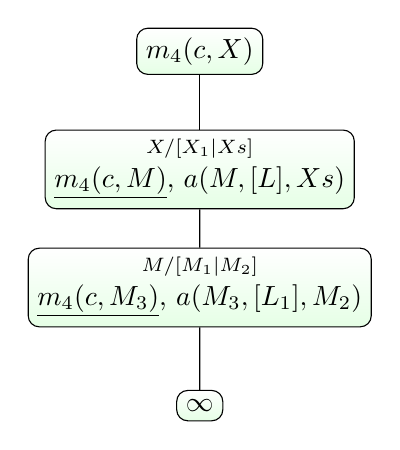
\begin{tikzpicture}[sibling distance=12em, align=center,
  every node/.style = {shape=rectangle, rounded corners,
    draw, align=center,
    top color=white, bottom color=green!10},
    level 1/.style={sibling distance=4cm},
    level 2/.style={sibling distance=4.7cm}, 
    level 3/.style={sibling distance=2.5cm}, ]
    \node {$m_4(c,X)$}
    child { node {\scriptsize $X/[X_1|Xs]$\\\underline{$m_4(c, M)$}, $a(M, [L], Xs$)}
      child { node {\scriptsize $M/[M_1|M_2]$\\\underline{$m_4(c, M_3)$}, $a(M_3, [L_1], M_2)$}
        child { node {$\infty$}}
      }
    };
\end{tikzpicture}